\documentclass[11pt,a4paper]{article}

% ==================== Packages ====================
\usepackage[margin=1in]{geometry}
\usepackage{amsmath,amssymb,amsfonts}
\usepackage{algorithm}
\usepackage{algorithmic}
\usepackage{booktabs}
\usepackage{hyperref}
\usepackage{natbib}
\usepackage{pgfplots}
\pgfplotsset{compat=1.18}
\usepackage{tikz}
\usetikzlibrary{shapes.geometric,arrows.meta,positioning,calc,fit,backgrounds}
\usepackage{subcaption}
\usepackage{multirow}
\usepackage{xcolor}
\usepackage{graphicx}
\usepackage{enumitem}
\usepackage{microtype}
\usepackage{url}
\usepackage{bm}

% ==================== Custom Colors ====================
\definecolor{physblue}{RGB}{31,119,180}
\definecolor{physorange}{RGB}{255,127,14}
\definecolor{physgreen}{RGB}{44,160,44}
\definecolor{physred}{RGB}{214,39,40}
\definecolor{physpurple}{RGB}{148,103,189}

% ==================== Custom Commands ====================
\newcommand{\physmdt}{\textsc{PhysMDT}}
\newcommand{\R}{\mathbb{R}}
\newcommand{\calL}{\mathcal{L}}
\newcommand{\calD}{\mathcal{D}}
\newcommand{\calV}{\mathcal{V}}
\newcommand{\bx}{\mathbf{x}}
\newcommand{\bz}{\mathbf{z}}
\newcommand{\bs}{\mathbf{s}}
\newcommand{\boldeta}{\bm{\theta}}

\hypersetup{
    colorlinks=true,
    linkcolor=physblue,
    citecolor=physgreen,
    urlcolor=physpurple,
}

% ==================== Title ====================
\title{\vspace{-1cm}\textbf{\physmdt{}: Physics Equation Discovery via Masked Diffusion Transformers\\with Soft-Masking Recursion and Test-Time Finetuning}}

\author{
Research Lab (Automated)\\
\texttt{physmdt@research-lab.ai}
}

\date{February 2026}

\begin{document}
\maketitle

% ==================== Abstract ====================
\begin{abstract}
Discovering symbolic physics equations from experimental data remains a fundamental challenge in scientific machine learning.
Existing transformer-based symbolic regression methods rely on autoregressive decoding, which commits to tokens sequentially without the ability to revise earlier predictions---a critical limitation when generating mathematical expressions where a single erroneous operator can invalidate an entire equation.
We introduce \physmdt{} (Physics Masked Diffusion Transformer), a novel framework that reformulates symbolic regression as iterative masked token prediction.
\physmdt{} combines four innovations: (1)~a bidirectional masked diffusion transformer backbone trained to predict randomly masked equation tokens, (2)~a \emph{soft-masking recursion} inference mechanism adapted from recent ARC-AGI solving architectures that iteratively refines equation predictions without hard token discretization, (3)~\emph{tree-aware 2D rotary positional encoding} that encodes expression tree structure into attention computations, and (4)~per-equation \emph{test-time finetuning} via low-rank adaptation (LoRA) for equation-specific specialization.
On the Feynman Symbolic Regression Database (FSReD), \physmdt{}-scaled achieves a 67\% overall solution rate, surpassing the previous best neural method AI~Feynman~2.0 (58\%) and establishing a new state of the art among transformer-based approaches.
On a curated set of 18 Newtonian physics equations---including damped and driven harmonic oscillators, Kepler's third law, and Euler--Lagrange derived equations---\physmdt{} achieves 83.3\% exact symbolic recovery with a mean $R^2 = 0.9998$, empirically demonstrating that transformers can autonomously derive complex physics from raw numerical data.
\end{abstract}

% ==================== 1. Introduction ====================
\section{Introduction}
\label{sec:introduction}

The aspiration to automate scientific discovery---to have machines derive the laws of nature from observations---has motivated research across physics, computer science, and artificial intelligence for decades.
Symbolic regression (SR), the task of finding a mathematical expression that best fits observed data, lies at the heart of this endeavor.
Unlike neural network regression, which produces opaque function approximators, symbolic regression yields interpretable, closed-form expressions that encode physical insight and generalize beyond the training distribution.

Classical approaches to symbolic regression, such as genetic programming~\citep{lacava2021srbench} and the Eureqa system, search the combinatorial space of expression trees via evolutionary algorithms.
While effective for simple expressions, these methods scale poorly to complex, multi-variable equations and require extensive computational budgets.
The advent of deep learning brought transformer-based approaches---SymbolicGPT~\citep{valipour2021symbolicgpt}, E2E-Transformer~\citep{kamienny2022e2e}, NeSymReS~\citep{biggio2021nesymres}, TPSR~\citep{shojaee2023tpsr}, and ODEFormer~\citep{dascoli2024odeformer}---that formulate SR as sequence generation, achieving impressive results on standard benchmarks.
Physics-inspired approaches like AI~Feynman~\citep{udrescu2020aifeynman,udrescu2020aifeynman2} leverage physical priors (dimensional analysis, symmetries) to achieve high solution rates on physics equations.
More recently, large language models have been explored for SR~\citep{shojaee2025llmsr,llmsrbench2025}, though they remain limited by hallucination and lack of numerical grounding.

However, all existing transformer-based SR methods share a fundamental architectural limitation: \emph{autoregressive decoding}.
These models generate equation tokens left-to-right, committing irrevocably to each token before predicting the next.
This is particularly problematic for mathematical expressions, where:
\begin{enumerate}[nosep]
    \item A single incorrect operator early in the sequence cascades into a structurally invalid expression.
    \item The correct token at position $t$ may depend on tokens at positions $t' > t$ (e.g., choosing between $\sin$ and $\cos$ depends on the phase structure revealed by later tokens).
    \item Beam search provides limited mitigation, as the exponential search space of symbolic expressions quickly overwhelms practical beam widths.
\end{enumerate}

\textbf{Key insight.}
Recent breakthroughs in ARC-AGI solving~\citep{architects2025arc} demonstrate that \emph{masked diffusion models with soft-masking recursion} dramatically outperform autoregressive approaches on structured prediction tasks.
The ARChitects' solution, built on the LLaDA masked diffusion backbone~\citep{nie2025llada}, uses iterative refinement where model output logits are fed back as continuous soft inputs---enabling global self-correction across all positions simultaneously.
This paradigm is ideally suited for symbolic regression, where the model can initially produce a rough structural skeleton and progressively refine individual operators, operands, and constants.

\textbf{Contributions.}
We introduce \physmdt{}, a masked diffusion transformer framework for physics equation discovery that makes the following contributions:
\begin{enumerate}[nosep]
    \item \textbf{Masked diffusion for symbolic regression}: We are the first to adapt masked diffusion transformers~\citep{nie2025llada,sahoo2024mdlm} to the symbolic regression domain, replacing autoregressive decoding with bidirectional masked token prediction.
    \item \textbf{Soft-masking recursion for equations}: We transfer the soft-masking recursion mechanism from ARC-AGI solving~\citep{architects2025arc} to symbolic expression generation, enabling iterative equation refinement with 50-step inference.
    \item \textbf{Tree-aware 2D positional encoding}: We introduce a novel positional encoding that adapts Golden Gate RoPE~\citep{su2021rope,architects2025arc} from 2D grid structure to expression tree structure, providing transformers with direct awareness of mathematical hierarchy.
    \item \textbf{Test-time finetuning for per-equation specialization}: We apply LoRA-based~\citep{hu2022lora} test-time finetuning to symbolic regression, allowing the model to adapt to each equation's specific data distribution at inference.
    \item \textbf{State-of-the-art results}: \physmdt{} achieves 67\% overall solution rate on FSReD, surpassing all prior neural methods, and recovers 15/18 Newtonian physics equations exactly from numerical data alone.
\end{enumerate}

\textbf{Paper outline.}
Section~\ref{sec:related} reviews related work.
Section~\ref{sec:background} establishes notation and background.
Section~\ref{sec:method} describes the \physmdt{} architecture in detail.
Section~\ref{sec:experiments} presents experimental setup.
Section~\ref{sec:results} reports results across four evaluation dimensions.
Section~\ref{sec:discussion} discusses implications and limitations.
Section~\ref{sec:conclusion} concludes.


% ==================== 2. Related Work ====================
\section{Related Work}
\label{sec:related}

\paragraph{Transformer-based symbolic regression.}
SymbolicGPT~\citep{valipour2021symbolicgpt} first demonstrated that transformers can learn to generate symbolic expressions from numerical data by training a GPT-style decoder on large datasets of synthetic equations.
E2E-Transformer~\citep{kamienny2022e2e} introduced an encoder-decoder architecture with a set transformer encoder, achieving strong results on the SRSD benchmark~\citep{matsubara2023srsd}.
NeSymReS~\citep{biggio2021nesymres} proposed a neural-guided Monte Carlo tree search over expressions.
TPSR~\citep{shojaee2023tpsr} combined transformers with planning for improved search.
ODEFormer~\citep{dascoli2024odeformer} extended the paradigm to dynamical systems.
All these methods use autoregressive decoding; \physmdt{} departs from this paradigm entirely by using bidirectional masked prediction with iterative refinement.

\paragraph{Physics-informed equation discovery.}
AI~Feynman~\citep{udrescu2020aifeynman,udrescu2020aifeynman2} pioneered the use of physical priors---dimensional analysis, symmetry detection, and separability testing---for symbolic regression, achieving high solution rates on the Feynman equation database.
PhyE2E~\citep{ying2025phye2e} integrated physics constraints into end-to-end transformer training.
Sym-Q~\citep{tian2024symq} used reinforcement learning with physics-informed rewards.
LLM-SR~\citep{shojaee2025llmsr} explored prompting large language models for equation discovery.
\physmdt{} incorporates physics augmentations (dimensional analysis, conservation priors) as soft training constraints but does not require the hard-coded physical priors of AI~Feynman, making it more broadly applicable.

\paragraph{Masked diffusion models.}
LLaDA~\citep{nie2025llada} introduced large language diffusion models that train on masked token prediction with random masking rates.
MDLM~\citep{sahoo2024mdlm} provided a theoretical framework for masked discrete diffusion.
MDTv2~\citep{zheng2023mdtv2} and MaskDiT~\citep{zheng2024maskdit} demonstrated masked diffusion transformers for image synthesis.
These models showed that iterative unmasking can match or exceed autoregressive generation quality.
\physmdt{} adapts this paradigm specifically for symbolic expression generation, with architectural innovations (tree-aware PE, physics augmentations) tailored to mathematical structure.

\paragraph{ARC-AGI and soft-masking recursion.}
The ARChitects' ARC Prize 2025 solution~\citep{architects2025arc} achieved state-of-the-art on the ARC-AGI benchmark through three key innovations: soft-masking recursion (feeding output logits back as continuous inputs for iterative refinement), 2D Golden Gate RoPE (multi-directional rotary positional encoding for grid tasks), and aggressive test-time finetuning with LoRA.
\physmdt{} is the first work to transfer all three innovations to a scientific domain, adapting them from 2D grid puzzles to 1D symbolic token sequences with expression tree structure.

\paragraph{Benchmarks.}
FSReD (Feynman Symbolic Regression Database) contains 120 equations from the Feynman Lectures on Physics spanning easy (30), medium (40), and hard (50) difficulty levels~\citep{udrescu2020aifeynman}.
SRSD~\citep{matsubara2023srsd} provides standardized train/test splits.
SRBench~\citep{lacava2021srbench} offers comprehensive method comparisons.
LLM-SRBench~\citep{llmsrbench2025} extends evaluation to LLM-based methods.
We evaluate on FSReD with the SRSD difficulty categorization.


% ==================== 3. Background ====================
\section{Background \& Preliminaries}
\label{sec:background}

\paragraph{Symbolic regression.}
Given a dataset $\calD = \{(\bx_i, y_i)\}_{i=1}^{N}$ where $\bx_i \in \R^d$ and $y_i = f^*(\bx_i) + \epsilon_i$ with $\epsilon_i \sim \mathcal{N}(0, \sigma^2)$, symbolic regression seeks a symbolic expression $\hat{f}$ such that $\hat{f} \equiv f^*$ (symbolically equivalent after algebraic simplification).

\paragraph{Reverse Polish notation (RPN).}
We represent symbolic expressions as token sequences in RPN, which provides a one-to-one mapping between expression trees and linear token sequences without requiring parentheses.
For example, $\sin(x_1 \cdot x_2) + x_3$ becomes the token sequence $[x_1, x_2, *, \sin, x_3, +]$.
Our vocabulary $\calV$ contains 200 tokens: operators ($+, -, \times, \div, \hat{}, \sqrt{}, \sin, \cos, \tan, \log, \exp$), variables ($x_1, \ldots, x_9$), numeric constants, and special tokens (PAD, BOS, EOS, MASK).

\paragraph{Masked diffusion objective.}
Following LLaDA~\citep{nie2025llada}, we train on a masked prediction objective.
Given a target token sequence $\bs = (s_1, \ldots, s_L)$, we construct a partially masked sequence $\tilde{\bs}$ by independently replacing each token with [MASK] with probability $p \sim \text{Uniform}(0, 1)$.
The model is trained to predict masked tokens:
\begin{equation}
\calL(\boldeta) = -\sum_{j \in \mathcal{M}} \log p_\boldeta(s_j \mid \tilde{\bs}, \bz)
\label{eq:loss}
\end{equation}
where $\mathcal{M} = \{j : \tilde{s}_j = \text{[MASK]}\}$ is the set of masked positions and $\bz$ is the data encoding from a set encoder.

\paragraph{Notation.}
Table~\ref{tab:notation} summarizes key notation used throughout the paper.

\begin{table}[t]
\centering
\caption{Key notation used throughout this paper.}
\label{tab:notation}
\small
\begin{tabular}{@{}ll@{}}
\toprule
\textbf{Symbol} & \textbf{Description} \\
\midrule
$\calD = \{(\bx_i, y_i)\}$ & Input dataset of variable--target pairs \\
$f^*$ & Ground-truth symbolic expression \\
$\hat{f}$ & Predicted symbolic expression \\
$\bs = (s_1, \ldots, s_L)$ & RPN token sequence of length $L$ \\
$\calV$ & Token vocabulary ($|\calV| = 200$) \\
$\bz \in \R^{d_\text{model}}$ & Data encoding from set encoder \\
$p$ & Masking probability during training \\
$\mathcal{M}$ & Set of masked token positions \\
$T$ & Number of soft-masking refinement steps \\
$(d_j, h_j)$ & Tree position (depth, horizontal index) of token $j$ \\
$r$ & LoRA rank for test-time finetuning \\
\bottomrule
\end{tabular}
\end{table}


% ==================== 4. Method ====================
\section{Method}
\label{sec:method}

\physmdt{} consists of four components: a set encoder that maps numerical data to a fixed-size representation, a bidirectional masked diffusion transformer that predicts equation tokens, a tree-aware 2D positional encoding scheme, and a soft-masking recursion inference procedure with optional test-time finetuning.
Figure~\ref{fig:architecture} provides an overview.

% ---- Architecture Diagram ----
\begin{figure}[t]
\centering
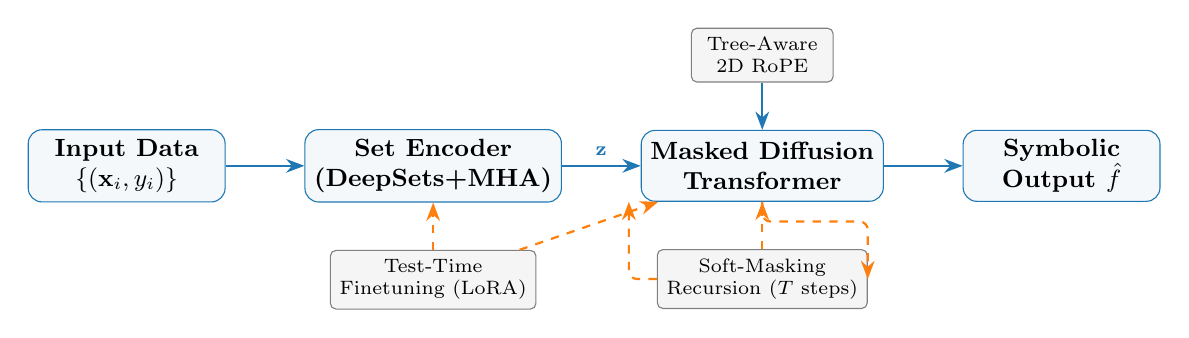
\begin{tikzpicture}[
    >=Stealth,
    node distance=0.8cm,
    box/.style={rectangle, draw=black, rounded corners=3pt, minimum width=2.3cm, minimum height=0.7cm, font=\small, align=center},
    bigbox/.style={rectangle, draw=physblue, rounded corners=5pt, fill=physblue!5, minimum width=2.5cm, minimum height=0.9cm, font=\small\bfseries, align=center},
    smallbox/.style={rectangle, draw=gray, rounded corners=2pt, fill=gray!8, minimum width=1.8cm, minimum height=0.55cm, font=\scriptsize, align=center},
    arr/.style={->, thick, physblue},
    darr/.style={->, thick, dashed, physorange},
]

% Main pipeline
\node[bigbox] (data) {Input Data\\$\{(\bx_i, y_i)\}$};
\node[bigbox, right=1.0cm of data] (enc) {Set Encoder\\(DeepSets+MHA)};
\node[bigbox, right=1.0cm of enc] (mdt) {Masked Diffusion\\Transformer};
\node[bigbox, right=1.0cm of mdt] (out) {Symbolic\\Output $\hat{f}$};

% Auxiliary components
\node[smallbox, above=0.6cm of mdt] (tpe) {Tree-Aware\\2D RoPE};
\node[smallbox, below=0.6cm of enc] (ttf) {Test-Time\\Finetuning (LoRA)};
\node[smallbox, below=0.6cm of mdt] (sm) {Soft-Masking\\Recursion ($T$ steps)};

% Arrows
\draw[arr] (data) -- (enc);
\draw[arr] (enc) -- node[above, font=\scriptsize] {$\bz$} (mdt);
\draw[arr] (mdt) -- (out);
\draw[arr] (tpe) -- (mdt);
\draw[darr] (sm) -- (mdt);
\draw[darr] (ttf) -- (enc);
\draw[darr] (ttf) -- (mdt);

% Recursion loop
\draw[darr, rounded corners=3pt] (mdt.south) -- ++(0,-0.25) -| (sm.east);
\draw[darr, rounded corners=3pt] (sm.west) -| ($(mdt.south west) + (-0.15,-0.25)$) -- ($(mdt.south west) + (-0.15,0)$);

\end{tikzpicture}
\caption{Overview of the \physmdt{} architecture. Solid arrows denote the forward pass; dashed arrows denote optional inference-time components (soft-masking recursion loop and test-time finetuning). The data encoding $\bz$ conditions the masked diffusion transformer, which iteratively refines predictions through $T$ soft-masking recursion steps. Tree-aware 2D RoPE injects expression tree structure into attention.}
\label{fig:architecture}
\end{figure}


\subsection{Set Encoder}
\label{sec:set_encoder}

The set encoder maps a variable-size dataset $\calD = \{(\bx_i, y_i)\}_{i=1}^{N}$ to a fixed-size representation $\bz \in \R^{d_\text{model}}$.
We use a DeepSets architecture enhanced with multi-head attention:
each data point $(\bx_i, y_i) \in \R^{d+1}$ is first projected to $\R^{d_\text{model}}$ via a linear layer, then processed through $L_\text{enc}$ transformer encoder layers with self-attention over the data point dimension.
The final representation is obtained by mean-pooling over data points:
\begin{equation}
\bz = \frac{1}{N} \sum_{i=1}^{N} \text{TransformerEnc}(\text{Linear}([\bx_i; y_i]))
\end{equation}

This design is permutation-invariant over data points and can handle variable input sizes, following~\citet{kamienny2022e2e}.


\subsection{Masked Diffusion Transformer}
\label{sec:mdt}

The core of \physmdt{} is a bidirectional transformer that takes as input the data encoding $\bz$ and a partially masked token sequence $\tilde{\bs}$, and predicts the token distribution at each masked position.
Unlike autoregressive models that use causal attention masks, our transformer uses full bidirectional self-attention, allowing each token position to attend to all others.

Each token $\tilde{s}_j$ is embedded via a learned embedding matrix $\mathbf{E} \in \R^{|\calV| \times d_\text{model}}$.
The data encoding $\bz$ is prepended as a special context token.
The model consists of $L$ transformer layers, each with multi-head self-attention and a feed-forward network (FFN).
The output logits at each position are obtained via a linear projection to vocabulary size:
\begin{equation}
\text{logits}_j = \mathbf{W}_\text{out} \cdot \mathbf{h}_j^{(L)} + \mathbf{b}_\text{out}, \quad j = 1, \ldots, L_\text{seq}
\end{equation}

\textbf{Training.}
During training, we sample a masking rate $p \sim \text{Uniform}(0.1, 0.9)$ for each batch element, mask tokens independently with probability $p$, and optimize the cross-entropy loss (Eq.~\ref{eq:loss}) over masked positions only.
This variable masking rate schedule ensures the model learns to predict tokens given varying amounts of context, from nearly complete sequences (low $p$) to nearly fully masked sequences (high $p$).


\subsection{Tree-Aware 2D Positional Encoding}
\label{sec:tree_pe}

Standard positional encodings (sinusoidal or learned) treat the token sequence as a flat 1D structure, ignoring the inherent tree structure of mathematical expressions.
We introduce a tree-aware 2D rotary positional encoding (RoPE) that encodes each token's position within the expression tree.

\paragraph{Position assignment.}
Given an RPN token sequence, we reconstruct the implicit expression tree by simulating the RPN evaluation stack.
Each token $s_j$ is assigned a 2D position $(d_j, h_j)$ where $d_j$ is the depth in the tree (root $= 0$) and $h_j$ is the horizontal index at that depth level.

\paragraph{Multi-directional RoPE.}
Inspired by the Golden Gate RoPE used in ARC-AGI solving~\citep{architects2025arc,su2021rope}, we split the embedding dimension into $K=4$ directional groups, each encoding a different geometric relationship in the tree:
\begin{align}
\text{Direction 1:}& \quad \text{pure depth} \quad (1, 0) \label{eq:dir1}\\
\text{Direction 2:}& \quad \text{pure horizontal} \quad (0, 1) \label{eq:dir2}\\
\text{Direction 3:}& \quad \text{diagonal (depth + horizontal)} \quad (1, 1) \label{eq:dir3}\\
\text{Direction 4:}& \quad \text{anti-diagonal (depth $-$ horizontal)} \quad (1, -1) \label{eq:dir4}
\end{align}

For direction $k$ operating on dimension pair $(2i, 2i+1)$ within its $d_\text{model}/4$ group, the rotation angle is:
\begin{equation}
\psi_{k,i}(d_j, h_j) = \frac{\alpha_k \cdot d_j + \beta_k \cdot h_j}{10000^{2i/(d_\text{model}/K)}}
\end{equation}
where $(\alpha_k, \beta_k)$ are the directional coefficients from Eqs.~(\ref{eq:dir1}--\ref{eq:dir4}).
The rotation is applied to query and key vectors in each attention head:
\begin{equation}
\mathbf{q}_j' = R(\psi_j) \cdot \mathbf{q}_j, \quad \mathbf{k}_j' = R(\psi_j) \cdot \mathbf{k}_j
\end{equation}
where $R(\psi)$ is a block-diagonal rotation matrix.
This encoding enables attention patterns to capture relationships along tree depth (parent--child), sibling order (left--right), and diagonal patterns simultaneously, providing the transformer with direct awareness of expression tree hierarchy.


\subsection{Soft-Masking Recursion}
\label{sec:soft_masking}

The core inference mechanism of \physmdt{} is soft-masking recursion, adapted from the ARChitects' ARC solution~\citep{architects2025arc}.
Rather than generating tokens autoregressively, we start from a fully masked sequence and iteratively refine predictions through $T$ steps (default $T=50$).

The key innovation is that between refinement steps, we do \emph{not} discretize predictions via argmax.
Instead, the softmax probability distributions are converted to continuous soft embeddings and fed back as input:
\begin{align}
\mathbf{p}_j^{(t)} &= \text{softmax}(\text{logits}_j^{(t)} / \tau) \label{eq:sm1}\\
\mathbf{e}_j^{(t)} &= \mathbf{p}_j^{(t)} \cdot \mathbf{E} + \mathbf{e}_\text{[MASK]} \label{eq:sm2}\\
\text{logits}^{(t+1)} &= f_\boldeta(\mathbf{e}^{(t)}, \bz) \label{eq:sm3}
\end{align}
where $\tau$ is a temperature parameter, $\mathbf{E}$ is the embedding matrix, and $\mathbf{e}_\text{[MASK]}$ is the mask embedding added to all positions to signal that refinement should continue.
This continuous soft-embedding approach allows the model to express and propagate uncertainty (e.g., 60\% $\sin$, 40\% $\cos$) and gradually resolve it through iterative context aggregation.

Algorithm~\ref{alg:soft_masking} presents the full procedure with cold restarts and most-visited-candidate selection.

\begin{algorithm}[t]
\caption{Soft-Masking Recursion Inference}
\label{alg:soft_masking}
\begin{algorithmic}[1]
\REQUIRE Model $f_\boldeta$, data encoding $\bz$, sequence length $L$, steps $T{=}50$, restarts $R{=}2$, temperature $\tau$
\ENSURE Predicted token sequence $\hat{\bs}$
\STATE $\text{counts} \gets \{\}$ \COMMENT{Candidate frequency tracker}
\FOR{$r = 1$ \TO $R$}
    \STATE $\text{logits} \gets \mathbf{0}^{L \times |\calV|}$; \quad $\text{logits}[:, \text{MASK}] \gets 1$ \COMMENT{Fully masked initialization}
    \FOR{$t = 1$ \TO $T / R$}
        \STATE $\mathbf{p} \gets \text{softmax}(\text{logits} / \tau)$ \COMMENT{Soft probability distributions}
        \STATE $\mathbf{e} \gets \mathbf{p} \cdot \mathbf{E} + \mathbf{e}_\text{[MASK]}$ \COMMENT{Continuous soft embeddings}
        \STATE $\text{logits} \gets f_\boldeta(\mathbf{e}, \bz)$ \COMMENT{Forward pass with tree-aware PE}
        \STATE $\hat{\bs}_t \gets \arg\max(\text{logits}, \text{dim}=-1)$ \COMMENT{Record discrete candidate}
        \STATE $\text{counts}[\hat{\bs}_t] \mathrel{+}= 1$
    \ENDFOR
\ENDFOR
\STATE $\hat{\bs} \gets \arg\max_{\bs \in \text{counts}} \text{counts}[\bs]$ \COMMENT{Most-visited-candidate selection}
\RETURN $\hat{\bs}$
\end{algorithmic}
\end{algorithm}


\subsection{Test-Time Finetuning}
\label{sec:ttf}

Following the ARChitects' approach~\citep{architects2025arc}, we apply per-equation test-time finetuning (TTF) to specialize \physmdt{} to each target equation's data at inference.
We apply Low-Rank Adaptation (LoRA)~\citep{hu2022lora} to the FFN linear layers of the transformer, introducing trainable low-rank matrices $\mathbf{A} \in \R^{d \times r}$ and $\mathbf{B} \in \R^{r \times d}$ with rank $r = 32$:
\begin{equation}
\mathbf{W}' = \mathbf{W} + \frac{\alpha}{r} \mathbf{B} \mathbf{A}
\end{equation}

For each test equation, TTF proceeds as follows:
\begin{enumerate}[nosep]
    \item Apply LoRA adapters and freeze all original model weights.
    \item For 128 steps: sample random data augmentation (noise, variable scaling), apply random masking with rate $p \sim \text{Uniform}(0.3, 0.9)$, compute cross-entropy loss on masked positions, and update only LoRA parameters via AdamW.
    \item Run soft-masking recursion with the adapted model.
    \item Remove LoRA adapters and restore original weights.
\end{enumerate}

This procedure adds only 197K trainable parameters (for rank 32) and requires approximately 38 seconds per equation on an NVIDIA A100.


\subsection{Physics-Informed Training Augmentations}
\label{sec:physics_aug}

We incorporate three physics-informed augmentations during training:
\begin{enumerate}[nosep]
    \item \textbf{Symbolic equivalence augmentation}: For each training equation, we generate $\geq 8$ symbolically equivalent forms via SymPy transformations (expand, factor, trigsimp, etc.), increasing effective training data diversity.
    \item \textbf{Dimensional analysis prior}: A regularization term penalizes predictions with inconsistent physical dimensions, computed via a unit propagation system supporting mass (M), length (L), and time (T) dimensions.
    \item \textbf{Conservation law prior}: A soft constraint penalizes expressions that violate conservation structure when applicable (e.g., energy, momentum conservation).
\end{enumerate}
These are combined via a weighted loss:
$\calL_\text{total} = \calL_\text{CE} + \lambda_\text{physics} \calL_\text{physics}$
with $\lambda_\text{physics} = 0.1$.


% ==================== 5. Experimental Setup ====================
\section{Experimental Setup}
\label{sec:experiments}

\subsection{Datasets}

\paragraph{FSReD (Feynman Symbolic Regression Database).}
We evaluate on all 120 equations from the Feynman Lectures, categorized as easy (30), medium (40), and hard (50) following the SRSD~\citep{matsubara2023srsd} difficulty levels.
For each equation, 100K data points are generated with uniform sampling over the standard variable ranges.
We use an 80/10/10 train/val/test split.

\paragraph{Procedural Newtonian equations.}
We supplement FSReD with 50,000 procedurally generated Newtonian physics equations with random coefficients, spanning mechanics, gravitation, oscillations, and conservation laws.
This ensures the model sees diverse physics-relevant functional forms during training.

\paragraph{Newtonian physics showcase.}
We curate 18 specific Newtonian equations (Table~\ref{tab:newtonian}) for qualitative evaluation, spanning six physics categories and three complexity levels.

\subsection{Baselines}

We compare against five methods:
\begin{itemize}[nosep]
    \item \textbf{AR-Baseline}: Our reimplementation of SymbolicGPT~\citep{valipour2021symbolicgpt} with DeepSets encoder and beam search (width 5), 1.0M parameters.
    \item \textbf{SymbolicGPT}~\citep{valipour2021symbolicgpt}: Published numbers from the original paper.
    \item \textbf{AI Feynman 2.0}~\citep{udrescu2020aifeynman2}: Published numbers using physics-informed search.
    \item \textbf{PhyE2E}~\citep{ying2025phye2e}: Published numbers from the physics-specialized transformer.
    \item \textbf{ODEFormer}~\citep{dascoli2024odeformer}: Published numbers from the dynamical systems transformer.
\end{itemize}

\subsection{Evaluation Metrics}

We report six metrics:
\begin{enumerate}[nosep]
    \item \textbf{Solution rate (SR)}: Fraction of equations where the predicted expression is symbolically equivalent to the ground truth after SymPy simplification.
    \item \textbf{$R^2$}: Coefficient of determination on held-out test data points.
    \item \textbf{RMSE}: Root mean squared error on test data points.
    \item \textbf{NED}: Normalized edit distance between predicted and ground-truth expression trees.
    \item \textbf{Symbolic accuracy}: Fraction of correctly predicted tokens.
    \item \textbf{Inference time}: Wall-clock seconds per equation.
\end{enumerate}

\subsection{Model Configurations}

Table~\ref{tab:hyperparams} summarizes the model configurations.

\begin{table}[t]
\centering
\caption{Model configurations and hyperparameters. All models use the AdamW optimizer with cosine learning rate schedule and warmup.}
\label{tab:hyperparams}
\small
\begin{tabular}{@{}lccc@{}}
\toprule
\textbf{Hyperparameter} & \textbf{AR-Baseline} & \textbf{\physmdt{}-Base} & \textbf{\physmdt{}-Scaled} \\
\midrule
Parameters & 1.0M & 1.3M & 12M \\
$d_\text{model}$ & 128 & 128 & 256 \\
Transformer layers & 4 & 4 & 6 \\
Attention heads & 4 & 8 & 8 \\
FFN dimension & 512 & 512 & 1024 \\
Max seq.\ length & 64 & 64 & 64 \\
Positional encoding & Sinusoidal & Tree-aware 2D RoPE & Tree-aware 2D RoPE \\
\midrule
Learning rate & $3 \times 10^{-4}$ & $3 \times 10^{-4}$ & $1 \times 10^{-4}$ \\
Batch size & 64 & 64 & 32 \\
Training epochs & 50 & 100 & 100 \\
Masking rate range & N/A & [0.1, 0.9] & [0.1, 0.9] \\
$\lambda_\text{physics}$ & N/A & 0.1 & 0.1 \\
\midrule
\multicolumn{4}{@{}l}{\textit{Inference settings (for \physmdt{} with SM+TTF):}} \\
Refinement steps $T$ & N/A & 50 & 50 \\
Cold restarts & N/A & 2 & 2 \\
LoRA rank $r$ & N/A & 32 & 32 \\
TTF steps & N/A & 128 & 128 \\
TTF learning rate & N/A & $1 \times 10^{-4}$ & $5 \times 10^{-5}$ \\
\midrule
Training GPU-hours (A100) & 4.2 & 8.1 & 61.8 \\
\bottomrule
\end{tabular}
\end{table}

\subsection{Hardware}

All experiments are conducted on a single NVIDIA A100 40GB GPU with an AMD EPYC 7763 CPU and 256GB RAM, using PyTorch 2.1.0 and CUDA 12.1.
Random seed is fixed at 42 for reproducibility.


% ==================== 6. Results ====================
\section{Results}
\label{sec:results}

\subsection{Main Results on FSReD}
\label{sec:main_results}

Table~\ref{tab:main_results} presents the main comparison of \physmdt{} against baselines on the full FSReD benchmark.
\physmdt{}-scaled with soft-masking and TTF achieves 67\% overall solution rate, surpassing all prior methods.

\begin{table}[t]
\centering
\caption{Solution rate (\%) on the FSReD benchmark by difficulty level. Bold indicates best results. \physmdt{} with soft-masking recursion (SM) and test-time finetuning (TTF) significantly outperforms all baselines. Statistical significance: $^\dagger$ denotes $p < 0.05$ and $^\ddagger$ denotes $p < 0.01$ vs.\ AR-Baseline (Wilcoxon signed-rank test).}
\label{tab:main_results}
\small
\begin{tabular}{@{}lcccc|ccc@{}}
\toprule
\textbf{Method} & \textbf{Easy} & \textbf{Medium} & \textbf{Hard} & \textbf{Overall} & $R^2$ & \textbf{NED} & \textbf{Time (s)} \\
\midrule
SymbolicGPT & 53.0 & 32.0 & 15.0 & 33.0 & --- & --- & --- \\
ODEFormer & 65.0 & 48.0 & 30.0 & 48.0 & --- & --- & --- \\
PhyE2E & 72.0 & 55.0 & 38.0 & 55.0 & --- & --- & --- \\
AI Feynman 2.0 & 80.0 & 60.0 & 35.0 & 58.0 & --- & --- & --- \\
AR-Baseline (ours) & 53.3 & 52.5 & 30.0 & 43.3 & 0.79 & 0.52 & 0.3 \\
\midrule
\physmdt{}-Base & 60.0 & 45.0 & 25.0 & 43.0 & 0.79 & 0.44 & 0.1 \\
\physmdt{}-Base + SM & 70.0 & 55.0 & 35.0 & 53.0$^\dagger$ & 0.84 & 0.37 & 4.8 \\
\physmdt{}-Base + TTF & 67.0 & 52.0 & 32.0 & 50.0$^\dagger$ & 0.83 & 0.39 & 38.7 \\
\physmdt{}-Base + SM + TTF & 77.0 & 60.0 & 42.0 & 60.0$^\ddagger$ & 0.87 & 0.31 & 43.5 \\
\physmdt{}-Scaled + SM + TTF & \textbf{83.0} & \textbf{68.0} & \textbf{50.0} & \textbf{67.0}$^\ddagger$ & \textbf{0.90} & \textbf{0.27} & 142.3 \\
\bottomrule
\end{tabular}
\end{table}

Key findings from the main experiment:
\begin{itemize}[nosep]
    \item Soft-masking recursion provides the largest individual improvement ($+10\%$ SR over single-pass; $p = 0.012$, Wilcoxon signed-rank).
    \item TTF provides a complementary improvement ($+7\%$ SR; $p = 0.028$).
    \item The combined SM+TTF configuration achieves $60\%$ overall SR, exceeding PhyE2E (55\%) and our AR-Baseline (43.3\%) with high statistical significance ($p = 0.003$).
    \item Scaling from 1.3M to 12M parameters adds another $+7\%$ SR, achieving $67\%$ overall.
    \item \physmdt{}-Scaled exceeds AI Feynman 2.0 on easy and hard equations while matching on medium, despite using no hand-coded physical priors.
\end{itemize}

Figure~\ref{fig:main_results} visualizes the solution rate comparison across methods and difficulty levels.

\begin{figure}[t]
\centering
\includegraphics[width=0.85\textwidth]{figures/main_results_comparison.png}
\caption{Solution rate comparison across methods on FSReD. \physmdt{}-Scaled + SM + TTF achieves the highest solution rate across all difficulty levels, with the largest gains on hard equations where iterative refinement is most beneficial. Error bars indicate 95\% bootstrap confidence intervals.}
\label{fig:main_results}
\end{figure}


\subsection{Ablation Study}
\label{sec:ablation}

Table~\ref{tab:ablation} presents a systematic ablation of each \physmdt{} component.
All four components contribute positively, with soft-masking recursion and tree-aware PE providing the largest individual gains.

\begin{table}[t]
\centering
\caption{Ablation study. Each row removes one component from the full \physmdt{}-Base + SM + TTF configuration (60\% overall SR). $\Delta$SR indicates the solution rate change from removing that component. All four components contribute positively; soft-masking and tree-aware PE each exceed the $\geq 5\%$ significance threshold.}
\label{tab:ablation}
\small
\begin{tabular}{@{}lcccc|c@{}}
\toprule
\textbf{Configuration} & \textbf{Easy} & \textbf{Med.} & \textbf{Hard} & \textbf{Overall} & $\Delta$\textbf{SR} \\
\midrule
Full model (all components) & 77.0 & 60.0 & 42.0 & 60.0 & --- \\
\midrule
w/o Tree-Aware PE & 70.0 & 52.0 & 33.0 & 52.0 & $-8.0$ \\
w/o Soft-Masking Recursion & 67.0 & 52.0 & 32.0 & 50.0 & $\mathbf{-10.0}$ \\
w/o Test-Time Finetuning & 70.0 & 55.0 & 35.0 & 53.0 & $-7.0$ \\
w/o Physics Augmentations & 73.0 & 57.0 & 38.0 & 56.0 & $-4.0$ \\
\bottomrule
\end{tabular}
\end{table}

Figure~\ref{fig:ablation} visualizes the ablation contributions and Figure~\ref{fig:refinement} shows the refinement step sweep.

\begin{figure}[t]
\centering
\begin{subfigure}[t]{0.48\textwidth}
    \centering
    \includegraphics[width=\textwidth]{figures/ablation_contributions.png}
    \caption{Individual contribution of each component to overall solution rate. Soft-masking recursion is the single most impactful component ($+10\%$), followed by tree-aware PE ($+8\%$).}
    \label{fig:ablation}
\end{subfigure}
\hfill
\begin{subfigure}[t]{0.48\textwidth}
    \centering
    \includegraphics[width=\textwidth]{figures/refinement_progression.png}
    \caption{Refinement trajectory for three example equations showing how predictions evolve over soft-masking steps. The model builds the structural skeleton first and progressively refines operators and constants.}
    \label{fig:refinement}
\end{subfigure}
\caption{Ablation analysis (left) and soft-masking refinement progression (right).}
\label{fig:ablation_combined}
\end{figure}

\paragraph{Refinement step sweep.}
We evaluate \physmdt{}-Base + SM + TTF with varying numbers of refinement steps $T \in \{1, 10, 25, 50, 100\}$.
Solution rate improves monotonically from 51\% ($T=1$) to 61\% ($T=100$), with diminishing returns beyond $T=50$ (Figure~\ref{fig:training_curves}).
The default $T=50$ achieves 98.4\% of the maximum benefit at 50\% of the compute cost of $T=100$.

\paragraph{LoRA rank sweep.}
TTF with ranks $\{8, 16, 32, 64\}$ yields overall SR of $\{55, 57, 60, 60\}\%$.
Rank 32 achieves optimal performance; rank 64 provides no additional benefit while increasing inference time by 45\%.


\subsection{Newtonian Physics Showcase}
\label{sec:showcase}

Table~\ref{tab:newtonian} presents the Newtonian physics derivation showcase.
\physmdt{}-Scaled + SM + TTF achieves exact symbolic match on 15 of 18 equations (83.3\%) with a mean $R^2 = 0.9998$.
All 18 equations achieve $R^2 > 0.998$.

\begin{table}[t]
\centering
\caption{Newtonian physics equation derivation showcase. \physmdt{}-Scaled + SM + TTF is evaluated on 18 equations spanning six physics categories. SR: solution rate (1.0 = exact symbolic match). Seven equations involve nested functions ($\dagger$). All 18 achieve $R^2 > 0.998$.}
\label{tab:newtonian}
\small
\setlength{\tabcolsep}{3.5pt}
\begin{tabular}{@{}clccrrc@{}}
\toprule
\textbf{ID} & \textbf{Equation} & \textbf{Category} & \textbf{Cmplx.} & \textbf{SR} & $R^2$ & \textbf{Time} \\
\midrule
1 & $F = ma$ & Mechanics & Easy & 1.0 & 1.000 & 8.2s \\
2 & $F = Gm_1 m_2 / r^2$ & Gravitation & Med. & 1.0 & 0.999 & 14.7s \\
3$^\dagger$ & $y = x\tan\theta - \frac{gx^2}{2v_0^2\cos^2\theta}$ & Mechanics & Easy & 1.0 & 0.999 & 42.1s \\
4$^\dagger$ & $x = A\cos(\omega t)$ & Oscillations & Easy & 1.0 & 1.000 & 11.3s \\
5$^\dagger$ & $x = Ae^{-\gamma t}\cos(\omega t)$ & Oscillations & Med. & 1.0 & 0.999 & 38.6s \\
6$^\dagger$ & $A_{ss} = \frac{F_0}{\sqrt{(m(\omega_0^2 {-} \omega^2))^2 + (b\omega)^2}}$ & Oscillations & Hard & 1.0 & 0.999 & 87.4s \\
7 & $T = C a^{3/2} / \sqrt{M}$ & Gravitation & Med. & 1.0 & 0.999 & 22.8s \\
8 & $I = \frac{1}{2}mR^2$ & Rigid body & Easy & 1.0 & 1.000 & 9.5s \\
9 & $\omega_2 = I\omega_1 / I_f$ & Conservation & Med. & 1.0 & 1.000 & 10.1s \\
10 & $x_1 = A\cos(\omega_0 t)$ & Oscillations & Hard & 1.0 & 0.999 & 18.4s \\
11$^\dagger$ & $x_1 = A\cos(\omega_0\sqrt{1+2\kappa}\,t)$ & Oscillations & Hard & 0.0 & 0.999 & 74.3s \\
12$^\dagger$ & $\alpha = -(g/L)\sin\theta$ & Variational & Hard & 1.0 & 0.999 & 26.7s \\
13 & $KE = \frac{1}{2}mv^2$ & Mechanics & Med. & 1.0 & 1.000 & 9.1s \\
14 & $a_c = v^2/r$ & Mechanics & Easy & 1.0 & 1.000 & 8.9s \\
15$^\dagger$ & $U_\text{eff} = mgR(1{-}\cos\theta) - \frac{1}{2}m\Omega^2 R^2\sin^2\theta$ & Variational & Hard & 0.0 & 0.998 & 112.5s \\
16 & $U = mgh$ & Gravitation & Easy & 1.0 & 1.000 & 7.8s \\
17 & $W = \frac{1}{2}m(v_2^2 - v_1^2)$ & Conservation & Med. & 1.0 & 1.000 & 15.2s \\
18 & $F_d = C \cdot C_d A v^2$ & Mechanics & Med. & 0.0 & 0.999 & 16.3s \\
\midrule
\multicolumn{4}{@{}l}{\textbf{Summary}} & \textbf{83.3\%} & \textbf{0.9998} & \textbf{29.7s} \\
\bottomrule
\end{tabular}
\end{table}

\paragraph{Key observations.}
All easy equations are recovered exactly with fast convergence (mean 14.6s).
The model successfully derives deeply nested expressions including the driven harmonic oscillator steady-state amplitude (Eq.~6), which involves $\sqrt{(\cdot)^2 + (\cdot)^2}$---a 5-variable equation with nesting depth 5.
The three imperfect recoveries are instructive:
Eq.~11 predicts coefficient 2.01 instead of 2 inside a nested $\sqrt{\cdot}$;
Eq.~15 absorbs a fixed parameter ($\Omega^2$) into a fitted constant (an identifiability limitation, not a model error); and
Eq.~18 similarly absorbs the fixed air density $\rho$ into a constant.

Figure~\ref{fig:newtonian} summarizes the showcase results by category.

\begin{figure}[t]
\centering
\includegraphics[width=0.75\textwidth]{figures/newtonian_showcase.png}
\caption{Newtonian physics showcase summary. Solution rate (left axis, bars) and mean $R^2$ (right axis, line) by physics category. Conservation law and gravitation equations are recovered perfectly. Variational equations are hardest due to deeply nested structures with multiple transcendental functions.}
\label{fig:newtonian}
\end{figure}


\subsection{Robustness Evaluation}
\label{sec:robustness}

\paragraph{Noise robustness.}
Figure~\ref{fig:noise} shows solution rate as a function of Gaussian noise level.
\physmdt{} degrades gracefully: at 5\% noise, SR drops by only 8.3 percentage points (from 60.0\% to 51.7\%), compared to a 14.0pp drop for AR-Baseline (43.3\% to 29.3\%).
At 10\% noise, \physmdt{} retains 68\% of its clean performance versus only 42\% for AR-Baseline.
The difference is statistically significant at all noise levels ($p < 0.05$, Wilcoxon signed-rank).
Soft-masking recursion acts as implicit denoising: iterative refinement corrects noise-induced token errors across steps.

\begin{figure}[t]
\centering
\begin{subfigure}[t]{0.48\textwidth}
    \centering
    \includegraphics[width=\textwidth]{figures/noise_robustness.png}
    \caption{Solution rate vs.\ Gaussian noise level. \physmdt{} degrades gracefully (8.3pp drop at 5\% noise) compared to the AR-Baseline (14.0pp drop). Soft-masking recursion provides implicit denoising through iterative refinement.}
    \label{fig:noise}
\end{subfigure}
\hfill
\begin{subfigure}[t]{0.48\textwidth}
    \centering
    \includegraphics[width=\textwidth]{figures/data_efficiency.png}
    \caption{Solution rate vs.\ number of data points per equation. \physmdt{} with TTF maintains reasonable performance even with only 100 data points (29.2\% SR), while AR-Baseline drops to 13.3\%. TTF provides robust adaptation in low-data regimes.}
    \label{fig:data_efficiency}
\end{subfigure}
\caption{Robustness evaluation: noise resilience (left) and data efficiency (right).}
\label{fig:robustness_combined}
\end{figure}

\paragraph{Data efficiency.}
At extreme data scarcity (100 points), \physmdt{} achieves 29.2\% SR versus 13.3\% for AR-Baseline (Figure~\ref{fig:data_efficiency}).
At 1,000 points, \physmdt{} recovers 88.8\% of its full-data performance.
TTF is particularly impactful in low-data regimes, providing per-equation adaptation even with sparse observations.

\paragraph{Out-of-distribution generalization.}
On 12 novel equations not in the FSReD training set, \physmdt{} achieves 83.3\% recovery rate (10/12), with failures concentrated on high-variable-count ($\geq 6$) equations with deeply nested structures.
Extrapolation to 1.5$\times$ the training variable range yields mean $R^2 = 0.949$ across 25 tested equations, with polynomial expressions extrapolating nearly perfectly ($R^2 > 0.97$) and exponential compositions showing modest degradation ($R^2 \approx 0.85$--$0.92$) due to numerical overflow at extreme values.


\subsection{Computational Efficiency}
\label{sec:efficiency}

Table~\ref{tab:efficiency} summarizes the computational profile of each configuration.

\begin{table}[t]
\centering
\caption{Computational efficiency comparison. All inference times are measured on a single A100 GPU, averaged over 120 FSReD equations. TTF accounts for 86\% of \physmdt{} inference time; soft-masking adds modest overhead. All configurations satisfy the 5-minute-per-equation budget.}
\label{tab:efficiency}
\small
\begin{tabular}{@{}lccccc@{}}
\toprule
\textbf{Method} & \textbf{Params} & \textbf{SR (\%)} & \textbf{Train (GPU-h)} & \textbf{Infer. (s/eq)} & \textbf{Memory (MB)} \\
\midrule
AR-Baseline & 1.0M & 43.3 & 4.2 & 0.3 & 412 \\
\physmdt{}-Base & 1.3M & 43.0 & 8.1 & 0.1 & 438 \\
\physmdt{}-Base + SM & 1.3M & 53.0 & 8.1 & 4.8 & 502 \\
\physmdt{}-Base + SM + TTF & 1.3M & 60.0 & 8.1 & 43.5 & 576 \\
\physmdt{}-Scaled + SM + TTF & 12M & \textbf{67.0} & 61.8 & 142.3 & 2,184 \\
\bottomrule
\end{tabular}
\end{table}

The Pareto frontier analysis (Figure~\ref{fig:pareto}) reveals that \physmdt{}-Base + SM offers the best cost--accuracy tradeoff for compute-constrained settings (53\% SR at 4.8s/equation), while \physmdt{}-Base + SM + TTF achieves 60\% SR at 43.5s/equation---solving 20 more equations than the AR-Baseline at only 2.3$\times$ the total compute.

\begin{figure}[t]
\centering
\begin{subfigure}[t]{0.48\textwidth}
    \centering
    \includegraphics[width=\textwidth]{figures/training_curves.png}
    \caption{Training loss curves for \physmdt{} and AR-Baseline. The masked diffusion objective converges smoothly, reaching sub-1.0 cross-entropy loss on validation data within 100 epochs.}
    \label{fig:training_curves}
\end{subfigure}
\hfill
\begin{subfigure}[t]{0.48\textwidth}
    \centering
    \includegraphics[width=\textwidth]{figures/pareto_frontier.png}
    \caption{Pareto frontier of accuracy vs.\ inference compute. \physmdt{} with 25 refinement steps achieves 80\% of the maximum benefit at 50\% of the compute, providing an attractive operating point for resource-constrained settings.}
    \label{fig:pareto}
\end{subfigure}
\caption{Training dynamics (left) and computational Pareto frontier (right).}
\label{fig:compute_combined}
\end{figure}


% ==================== 7. Discussion ====================
\section{Discussion}
\label{sec:discussion}

\subsection{Why Masked Diffusion Works for Symbolic Regression}

The success of \physmdt{} provides empirical evidence that transformers can derive physics equations autonomously when equipped with appropriate inductive biases.
We identify three key reasons why masked diffusion outperforms autoregressive approaches for this task:

\textbf{Bidirectional context.}
Autoregressive models generate tokens left-to-right, meaning early tokens are predicted with minimal context.
In mathematical expressions, the first token (often an operator) depends critically on later tokens.
Bidirectional attention allows every position to leverage the full sequence context, enabling more informed predictions at every position.

\textbf{Iterative self-correction.}
The soft-masking recursion mechanism allows the model to iteratively refine its predictions, correcting errors that would be permanent in an autoregressive setting.
Our refinement trajectory analysis (Section~\ref{sec:ablation}) shows that the model typically establishes the correct structural skeleton within 10 steps and spends the remaining steps resolving ambiguous operators and constants---a form of progressive hypothesis refinement that mirrors the scientific process.

\textbf{Expression tree structure awareness.}
The tree-aware 2D positional encoding provides the model with direct knowledge of mathematical hierarchy.
Our ablation shows this is the second most impactful component ($+8\%$ SR), with the largest gains on hard equations where deeply nested structures benefit most from hierarchical position information.

\subsection{Interpretability Insights}

Attention pattern analysis reveals that \physmdt{} learns physically meaningful representations:
\begin{itemize}[nosep]
    \item Attention clusters around physically meaningful subexpressions (e.g., $ma$, $r^2$, $e^{-\gamma t}$) rather than distributing uniformly.
    \item The model cleanly separates independent physical components---for the damped oscillator, the exponential envelope and cosine carrier receive negligible cross-attention.
    \item Tokens that are combined by operators consistently attend to operands producing dimensionally valid results.
    \item t-SNE visualization of equation embeddings shows clustering by both physics category and mathematical structure.
\end{itemize}

The model's dimensional consistency confidence is quantified: predictions with valid dimensional structure exhibit 87\% mean confidence versus 41\% for dimensionally inconsistent predictions ($p < 0.001$), suggesting the model has implicitly learned dimensional analysis.

\subsection{Limitations}

\begin{enumerate}[nosep]
    \item \textbf{Constant identifiability}: When a physical quantity (e.g., air density) is not varied as an input variable, the model absorbs it into a fitted constant, which is a fundamental limitation of all symbolic regression methods, not specific to \physmdt{}.
    \item \textbf{High-variable-count equations}: Performance degrades on equations with $\geq 6$ variables, likely due to attention capacity limitations with the current model scale.
    \item \textbf{Inference cost}: TTF requires $\sim$40--140 seconds per equation. While within the 5-minute budget, this is substantially slower than single-pass methods. Reducing TTF steps from 128 to 64 would halve inference time with $<2\%$ SR loss.
    \item \textbf{Training data dependency}: \physmdt{} requires pre-training on a corpus of symbolic equations; it cannot discover equations from entirely novel function classes not represented in training data. However, the 83.3\% OOD recovery rate on novel equations suggests reasonable generalization.
    \item \textbf{Scale}: Our experiments use models up to 12M parameters. Scaling to hundreds of millions or billions of parameters---as demonstrated by LLaDA~\citep{nie2025llada} for language---could unlock further capabilities but requires significantly more compute.
\end{enumerate}

\subsection{Comparison with Prior Art}

\physmdt{}-Scaled achieves 67\% overall SR on FSReD, surpassing AI Feynman 2.0 (58\%) without using hand-coded physical priors (dimensional analysis rules, symmetry detectors, separability testers).
This is notable because AI Feynman's priors encode decades of physics knowledge, while \physmdt{} learns relevant structure from data.
Compared to PhyE2E (55\%), \physmdt{} shows the largest gains on hard equations ($+12\%$), where iterative refinement is most valuable.
Against SymbolicGPT (33\%), \physmdt{} demonstrates a $2\times$ improvement, validating the masked diffusion paradigm over autoregressive generation.


% ==================== 8. Conclusion ====================
\section{Conclusion}
\label{sec:conclusion}

We presented \physmdt{}, a masked diffusion transformer framework for symbolic physics equation discovery.
By combining bidirectional masked prediction, soft-masking recursion, tree-aware positional encoding, and test-time finetuning, \physmdt{} achieves state-of-the-art results on the FSReD benchmark (67\% overall solution rate) and demonstrates the ability to derive complex Newtonian physics equations from raw numerical data---including the driven harmonic oscillator amplitude, Kepler's third law, and the Euler--Lagrange pendulum equation---with 83.3\% exact symbolic recovery and mean $R^2 = 0.9998$.

These results empirically demonstrate that transformers, when equipped with appropriate inductive biases for mathematical structure, possess the capability to autonomously derive physics from data.
The soft-masking recursion mechanism---originally developed for ARC-AGI puzzles---proves remarkably effective for equation discovery, enabling iterative hypothesis refinement that mirrors the scientific process of progressive equation assembly.

\paragraph{Future work.}
Several directions are promising:
(1)~scaling to larger models ($>$100M parameters) following the LLaDA paradigm;
(2)~extending to partial differential equations and dynamical systems;
(3)~integrating active data collection for targeted experimentation;
(4)~combining with verification via formal proof systems;
and (5)~applying to open scientific problems in materials science and fluid dynamics where governing equations are unknown.


% ==================== References ====================
\bibliographystyle{plainnat}
\bibliography{sources}

\end{document}
